%TC: macro \marginfootnote [other]
%TC: envir SCfigure [] other
%TC: macrocount beginSCfigure [figure]
\documentclass[11pt,twoside]{report}
\usepackage{preamble}
\setcounter{chapter}{5}
\graphicspath{{../img/}}
\def\includebibliography{}

\externaldocument{background}
\externaldocument{supercooled-liquids}
\externaldocument{morphometric-framework}
\externaldocument{appendix-spt-singularities}

\begin{document}
\chapter{Morphological thermodynamics for hard bodies from a controlled expansion}
\epigraph{He said that the geometry of the dream-place he saw was abnormal, non-Euclidean, and loathsomely redolent of spheres and dimensions apart from ours.}{H.\ P.\ Lovecraft, \emph{The Call of Cthulhu} (1926).}
\label{chapter:resummation}

This is the final chapter on the morphometric approach, but has a different focus from the previous two.
Here we derive the morphometric approach from first-principles in the case of hard particle systems, to place it on more rigorous footing and potentially indicate how the approximation may be improved.
We intend to publish part of this work at a later time as Ref.\ \cite{RobinsonResummation2019}.

\section{Introduction}

The standard theoretical framework for treating inhomogeneous liquids is classical density functional theory (DFT), which we introduced in section \ref{sec:dft}.
Central to this theory is the result that the free energy can be \emph{exactly} expressed as a functional of the density $\Omega = \Omega[\rho(\vec{r})]$ \cite{EvansAP1979}, though approximate functionals must be used in general.
For example, fundamental measure theory (FMT) \cite{RosenfeldPRL1989} provides a class of highly accurate functionals for the hard sphere liquid (cf.\ section \ref{sec:fmt}).
% relying on physical ingenuity.
A common practical application of DFT is to its \emph{dual} problem: determining the free energy $\Omega = \Omega[\phi_\mathrm{ext}(\vec{r})]$ for a fixed external potential $\phi_\mathrm{ext}(\vec{r})$.
Approaching this through DFT requires minimisation of $\Omega$ to obtain the equilibrium density profile, a tractable but expensive procedure.
In situations where many function evaluations are required, e.g.\ when integrating over many different realisations of $\phi_\mathrm{ext}$, this minimisation operation can become prohibitively expensive.
It is worthwhile to investigate more direct routes to approximating $\Omega[\phi_\mathrm{ext}(\vec{r})]$, especially where accuracy may be less important than fast calculation.

Unsurprisingly, we advocate the morphometric approach of previous chapters as a promising alternative to the dual problem outlined above, which has the potential to enable fast and accurate calculations in hard spheres \cite{RothPRL2006,Hansen-GoosPRL2007,RobinsonPRL2019}.
The morphometric approach concerns sharply repulsive external potentials where $\phi_\mathrm{ext}$ acts as a container for the fluid or as an exclusion volume for e.g.\ a solute.
In this limit, the density profile is negligible over a volume $V$ and the free energy is expanded in terms involving $V$ and its boundary $\partial V$.
We have hitherto focused on the morphometric approach in three dimensions%
\marginfootnote{See \eqref{eq:fmt-morphometric} for the morphometric approach as a limit of FMT, or \eqref{eq:morph-ansatz} as a generalisation of scaled particle theory.},
but in this chapter we will examine its fundamental basis and we will find it useful to consider the $d$-dimensional generalisation.
Motivated by integral geometry, we approximate the free energy change due to the inhomogeneous potential $\Delta \Omega := \Omega[\phi_\mathrm{ext}] - \Omega_\mathrm{hom}$ as the \emph{strictly extensive} quantity
\begin{equation}\label{eq:morphometric-approach-d}
  \Delta \Omega
  =
  \sum_{k=0}^d a_k V_k,
\end{equation}
with $V_k$ as the intrinsic volumes of the region defined by $\phi_\mathrm{ext}$.
This form of the grand potential is motivated by Hadwiger's characterisation theorem \eqref{eq:extensive-integral-geometry-d}.
%% \begin{equation}\label{eq:morphometric-approach}
%%   %\Omega[\phi_\mathrm{ext}] - \Omega_\mathrm{hom}
%%   \Delta \Omega
%%   =
%%   p V + a_2 A + a_1 C + a_0 X,
%% \end{equation}

Despite its accuracy in hard spheres, the morphometric expansion \eqref{eq:morphometric-approach-d} is still an approximation as has been demonstrated in numerous detailed investigations \cite{OettelEL2009,AshtonPRE2011,LairdPRE2012,BlokhuisPRE2013,UrrutiaPRE2014,Hansen-GoosJCP2014}.
Fundamental questions remain over \emph{why} it is accurate and how one might improve the approximation.
Inaccuracies become significant in hard spheres at very high densities approaching the glass transition, as we have seen in previous chapters, so an approximation scheme including additional terms could be desirable.
In this chapter we will attempt to start the path towards supplementing the morphometric approach \eqref{eq:morphometric-approach-d} with higher-order terms, by deriving the known terms as the leading contribution in the only properly rigorous free energy expansion: the \emph{virial series} introduced in section \ref{sec:virial-series}.
This route suggests a properly controlled way of including successive corrections to the approach.

Traditionally, expansions of $\Delta \Omega$ have been obtained in an \emph{ad-hoc} way rather than as part of a controlled expansion.
To illustrate this we consider what happens if one attempts to extend \eqref{eq:morphometric-approach-d} by including higher moments of curvature.
A prototypical example of this is the \emph{Helfrich expansion} for elastic membranes \cite{HelfrichZFNC1973}, which is often argued to be the most general expansion for the surface tension \cite{BlokhuisPRE2013}.
In this expansion, the next leading order correction to \eqref{eq:morphometric-approach-d} would be%
\marginfootnote{We remind the reader that $H(\vec{r})$ is the mean curvature along the surface, in the notation we used to introduce the key geometric quantities of integral geometry in $d=3$ in \eqref{eq:intrinsic-volumes-surface-integrals}.}
\begin{equation*}
  \int_{\partial V} H(\vec{r})^2 d\vec{r},
\end{equation*}
which is not well-defined for general surfaces, in particular for surfaces containing vertices and/or arcs as occurs in e.g.\ polyhedra.
To demonstrate this we consider the line where two planes intersect with dihedral angle $\Delta \theta$.
This can be considered as a cylindrical sector in the limit of vanishing radius $r$, giving the contribution per unit length
\begin{equation*}
  \int H^2 r d\theta
  = \frac{\Delta \theta}{r}
\end{equation*}
diverging as $1 / r$ in the limit where the sector becomes an arc $r \to 0$.
By contrast, the geometric terms already present in the morphometric approach remain well defined even where a curvature tensor is not locally definable, at e.g.\ a cusp.
%this property is central to the success of the expansion \eqref{eq:morphometric-approach-d} so that the coefficients can be independent of the geometry.
Thus, the coefficients of any higher-order moments of curvature must necessarily be zero within a controlled expansion.
The inclusion of higher-order curvatures was originally motivated by continuum elasticity \cite{HelfrichZFNC1973}, so it is not surprising that features on small lengthscales are pathological.

More generally, we find that \emph{any} analytic geometric expansion of $\Delta \Omega$ cannot be exact.
It was shown in the original papers on scaled particle theory \cite{ReissJCP1959,ReissJCP1960} that $\Delta \Omega$ contains singularities, which cannot be captured by simple geometric expansions; we recount this argument in Appendix \ref{appendix:spt-singularities}.
The virial series is in principle exact, so any singularities should be captured by resumming its terms which could suggest forms for new approximation schemes.
%Correspondingly, proposed approximations of $\Omega[\phi_\mathrm{ext}(\vec{r})]$ which do not share this feature can be ruled out as general expansions.

%% Our argument can be summarised by.
%% This is not a surprising fact in itself as the morphometric approach can be obtained as a limit case of FMT \cite{Hansen-GoosJPCM2006}.
%% Our central argument is that the strength of the morphometric approach comes from underlying agreement with the leading contributions in the (exact) virial expansion, so a proper extension should be rooted in the virial series.
%% Homogeneous is simpler, so extensions may be possible where they are not in the inhomogeneous case.

%% To do this we will explore how this approach emerges from the virial expansion and what form it takes for other shapes and mixtures.
%% The virial expansion provides a few exact results which can be used to explore the limitations of approximate theories.

In sections \ref{sec:low-densities} and \ref{sec:hard-rods} we will present the limiting cases where the insertion cost rigorously takes the morphometric form, i.e.\ the low density limit and for one-dimensional hard rods.
In section \ref{sec:finite-densities} we resum the terms contributing in these exact limits to obtain a piece of the solvation energy which \emph{exactly} obeys the morphometric form, and we are able to calculate the thermodynamic coefficients explicitly.
Our main result is valid for hard interactions where the solute and solvent particles are comapct and convex.
Though applicable to arbitrary mixtures of particle geometries, the resulting form is equivalent to the standard morphometric approach \eqref{eq:morphometric-approach-d}.
The methods we use are identical to those used in analysis of inhomogeneous FMT, reflecting the deep underlying connections between FMT and the morphometric approach \cite{LeithallPRE2011,KordenPRE2012,MarechalPRE2014}.

%% The motivation for doing this is primarily to justify the morphometric approach by demonstrating that additional contributions are small for hard spheres, and from this develop an understanding of where the approach may fail.
%% The analytical thermodynamic coefficients we obtain provide a starting point for modelling new systems where a theory may not be available.
%% Furthermore, we use the form of the exact contribution to argue that the generalisation to mixtures suggested in \eqref{eq:morphometric-approach-mixtures} is unnecessary, as the exact contribution has the simpler form of \eqref{eq:morphometric-approach}.
%% Finally, the framework we use to obtain this contribution is \emph{identical} to the virial expansion approach for FMT; this approach has been systematically explored in the more general case of inhomogeneous systems \cite{LeithallPRE2011,KordenPRE2012,MarechalPRE2014}.
%% By applying this approach to our much simpler (essentially homogeneous) system we hope to make the ideas and techniques more accessible.

%% Historically, the morphometric approach has been argued on the grounds laid out above, and as a limiting case of FMT.
%% The goal in subsequent sections will be to review the many arguments to understand why it works, reveal its limitations and inform better approximation schemes.
%% FMT is not needed to justify the morphometric approach, although the two theories are deeply related by the same underlying geometric framework.

%% In section \ref{sec:singularities} we show that the cost of inserting a solute is not necessarily analytic, so an expansion in terms of geometrical properties will only be approximate in general.

\section{Exact morphometric limits}

\subsection{One-dimensional hard rods}
\label{sec:hard-rods}

The one-dimensional analogue of a hard sphere is a hard rod%
\marginfootnote{In fact, rods are the only convex shape possible in 1d (as line segments) so they are really the one-dimensional analogue of \emph{any} convex object.}.
The cost of inserting a new rod of length $L$ exactly fits the morphometric form independent of density.

Imagine a hard rod liquid occupying all of space.
If we insert a single fixed hard point at the origin, this splits the liquid into two half spaces on either side of the origin, i.e.\ $x < 0$ (left) and $x > 0$ (right).
Because the interactions are hard the two half spaces will be completely decorrelated; thus, growing the point to become a rod of finite size $L$ will simply correspond to translating one of the spaces a distance $L$ requiring work $p L$.
In the limit $L \to 0$ where the rod becomes a point there will be a fixed insertion cost
\begin{equation*}
  \beta \Delta \Omega(L=0) = -\ln{(1-\eta)}
\end{equation*}
coming from the fact that the probability that a randomly chosen position is unoccupied is simply the free volume $1-\eta$ \cite{ReissJCP1959}.
Combining these two terms gives the total cost of inserting a finite sized rod as
\begin{equation}\label{eq:hard-rods-morphometric}
  \beta \Delta \Omega(L) = \beta p L - \ln{(1-\eta)}
\end{equation}
which is exactly of morphometric form (cf.\ \eqref{eq:extensive-integral-geometry-d}).
The pressure can be determined as \cite{TonksPR1936}
\begin{equation}\label{eq:hard-rods-eos}
  \frac{\beta p}{\rho} = \frac{1}{1 - \eta}.
\end{equation}

The morphometric form is violated when multiple rods are inserted at such a distance apart that a liquid is confined between them.
In this case long-range correlation effects form between the rods which are not captured by the geometric expansion.

\subsection{Low densities in arbitrary dimensions}
\label{sec:low-densities}

We will now obtain the low density asymptotics of the chemical potential, and show that this exactly follows the morphometric form for convex bodies.
This argument is very similar to the one we used in the introduction of FMT in section \ref{sec:fmt}, and an argument from Ref.\ \cite{WertheimMP1994}.

Hard particles feature purely geometric interactions, a property that allows us to make progress.
In particular, the interaction potential between two compact and convex hard bodies $A,B \in \mathcal{K}^d$ is normally written
\begin{equation*}\label{eq:hard-mayer-f}
  u(A,B)
  =
  \begin{cases}
    0 & \textrm{ if } A \cap B = \emptyset \\
    \infty & \textrm{ if } A \cap B \ne \emptyset
  \end{cases}
\end{equation*}
from which the Mayer function \eqref{eq:mayer-function} can be written in the revealing form
\begin{equation*}\label{eq:hard-mayer-f}
  -f_{AB}
  =
  1 - e^{-\beta u(A,B)}
  =
  \begin{cases}
    0 & \textrm{ if } A \cap B = \emptyset \\
    1 & \textrm{ if } A \cap B \ne \emptyset
  \end{cases}
\end{equation*}
The latter form is identical in form to the Euler characteristic, introduced in \eqref{eq:euler-characteristic-definition}, of their intersection i.e.\
\begin{equation*}
  \chi[A \cap B] =
    \begin{cases}
    0 & \textrm{ if } A \cap B = \emptyset \\
    1 & \textrm{ if } A \cap B \ne \emptyset
    \end{cases}
\end{equation*}
valid for convex bodies.
Comparing this expression with \eqref{eq:hard-mayer-f} we can rewrite the thermodynamic quantity as the purely geometrical measure
\begin{equation}\label{eq:chi-replacement}
  1 - e^{-\beta u(A,B)} = \chi[A \cap B] = -f_{AB}.
\end{equation}
Rewriting the interactions in terms of the Euler characteristic allows us to exploit theorems from integral geometry to evaluate thermodynamic quantities.

Including their relative orientations, the cost of inserting a solute $A$ into a liquid of $B$ particles in the low density limit $\rho \ll 1$ is determined from leading contribution in the virial series using \cite{Hansen2013,Santos2016}
\begin{equation}\label{eq:low-density-insertion}
  \begin{split}
    \beta\Delta\Omega
    &=
    \frac{\rho}{2}
    \mayerdiagram[|][t.]{2}
    %% \frac{\rho}{2} \int_{G_d} \left( 1 - e^{-\beta u(A, gB)} \right) dg
    + \mathcal{O}(\rho^2)
    \\ &=
    \frac{\rho}{2} \int_{G_d} \chi[A \cap gB] dg
    + \mathcal{O}(\rho^2)
  \end{split}
\end{equation}
where we indicate the $A$ particle with a triangle and the $B$ particle by a circle in the diagram, and we made the replacement \eqref{eq:chi-replacement} in the second line.
The integrand in the latter line of \eqref{eq:low-density-insertion} can be directly evaluated using the principal kinematic formuala \eqref{eq:binomial-kinematic-formula} giving the morphometric form \eqref{eq:morphometric-approach-d} with coefficients
\begin{equation*}
  a_k = \frac{V_{d-k}[B]}{C_{k,d-k}},
\end{equation*}
with coefficients $C_{k,d-k}$ defined in \eqref{eq:flag-coefficients}.
Thus the morphometric approach is exact in the low density limit.
This leads to elegant formulae e.g.\ for $d = 3$ we obtain
\begin{equation*}\label{eq:low-density-morphometric-result}
  \frac{\beta \Delta \Omega}{2 \pi \rho} =
  V[A] X[B] + A[A] C[B] + C[A] A[B] + X[A] V[B]
\end{equation*}
for $\rho \ll 1$, where we have used normalisations of intrinsic volumes as surface measures given in \eqref{eq:intrinsic-volumes-surface-integrals} and Table \ref{table:geometric-quantities}.
The low density result is a classic application of integral geometry to the liquid state, first obtained by Isihara \cite{IsiharaJCP1950}.

\section{Extension to finite densities in arbitrary dimensions}
\label{sec:finite-densities}

We can identify the insertion cost of a solute particle with the chemical potential of a new species of particle (a single solute) in the infinitely dilute limit \cite{ReissJCP1959,Hansen-GoosJPCM2006,Hansen-GoosJCP2014}.
Interestingly, taking this limit for a bulk hard sphere system modelled with fundamental measure theory (FMT) gives the morphometric approach (cf.\ section \ref{sec:fmt} and Ref.\ \cite{Hansen-GoosJPCM2006}); this is due to the approximation underlying FMT is that the free energy density can be represented in terms of weighted densities, which are deeply connected to intrinsic volumes.
Alternatively, the exact free energy of this system can be expressed as a virial expansion \cite{Hansen2013}.
This idea was explored in Ref.\ \cite{Hansen-GoosJPCM2006} to show that the morphometric approach \eqref{eq:morphometric-approach-d} is inexact, however here we will attempt a different strategy: we will identify a contribution in the virial expansion which guarantees an insertion cost of morphometric form.
The remaining contributions are unlikely to be rigorously of this form, and their omission is an approximation.

We consider an $(m+1)$-component mixture and we label each species with index $s \in \{0, 1, \cdots, m\}$: the components labelled $\{1, \cdots, m\}$ make up those species present the bulk liquid while the additional component with index $\{0\}$ represents the solute.
Furthermore, we assume each particle in this mixture is a compact and convex body $K_0, K_1, \cdots K_m \in \mathcal{K}^d$.
We will shortly find the chemical potential of the solute by considering the infinitely dilute limit.
For convenience, we restate the virial series for the excess free energy density \eqref{eq:free-energy-density} here as
\begin{equation}
  %% \beta f^\mathrm{ex}
  %% :=
  \frac{\beta F^\mathrm{ex}}{V}
  =
  \sum_{n=2}^\infty
  \frac{1}{n-1}
  B_n
  \rho^n,
\end{equation}
and restating the $n$th virial coefficient \label{eq:virial-coefficients-mixtures} as
\begin{equation}
  B_n
  =
  \sum_{s_1=0}^m \cdots \sum_{s_n=0}^m
  B_{s_1, \cdots, s_n} \prod_{i=0}^n x_{s_i},
\end{equation}
where $x_i$ is the mole fraction of species $i$ such that $x_i > 0$ and $\sum_{i=0}^m x_i = 1$.
$B_{s_1, \cdots, s_n}$ are the composition independent virial coefficients describing the contribution from interactions between $n$ particles of species $\{s_0, s_1, \cdots, s_n\}$.
Each contribution contains integrals over all configurations of the $n$ particles \cite{Hansen2013,Santos2016}.
We will refer to these contributions as diagrams because they are normally represented using graph theoretic tools such as when they were introduced in section \ref{sec:virial-series}.

We now identify the insertion cost for a new solute particle with its chemical potential in the dilute limit.
The chemical potential of the solute species is
\begin{equation}  
  \beta \mu^\mathrm{ex}_0
  =
  \frac{1}{\rho}
  \frac{\partial}{\partial x_0}
  \left( \frac{\beta F^\mathrm{ex}}{V} \right)_{V,T}
\end{equation}
giving in the dilute limit $x_0 \ll \rho$
\begin{equation}\label{eq:chemical-potential-mixture}
  \begin{split}
    \beta \Delta\Omega
    &=
    \lim_{\substack{x_0 \to 0}}
    \sum_{n=2}^\infty
    \frac{1}{n-1}
    \frac{\partial B_n}{\partial x_0}
    \rho^{n-1}
    \\
    &=
    \sum_{n=2}^\infty
    \frac{n}{n-1}
    B_{n-1}^*
    \rho^{n-1}
    =
    \sum_{n=1}^\infty
    \frac{n+1}{n}
    B_n^*
    \rho^n
  \end{split}
\end{equation}
with modified virial coefficient
\begin{equation}
  B_n^* =
  \sum_{s_1=1}^m \cdots \sum_{s_n=1}^m
  B_{0, s_1, \cdots, s_n}
  \prod_{i=1}^n x_{s_i}
\end{equation}
which contains contributions from all diagrams including a single member of the solute species.
In a single-component system we obtain the first few terms as \cite{Santos2016}
\begin{subequations}
  \begin{align}
    B_2
    &=
    - \frac{1}{2} \mayerdiagram[|][t.]{2},
    \\
    B_3
    &=
    - \frac{2}{3!} \mayerdiagram[|||][t..]{3},
    \\
    B_4
    &=
    - \frac{3}{4!}
    \left(
    3 \mayerdiagram[|.||.|][t...]{4}
    + 3 \mayerdiagram[|.||||][t...]{4}
    + 3 \mayerdiagram[||||.|][t...]{4}
    + \mayerdiagram[||||||][t...]{4}
    \right)
  \end{align}
\end{subequations}
using the diagrammatic notation for the integrals introduced in section \ref{sec:virial-series} with the small modification being that the solute is represented by a triangle.

We now introduce our central approximation which generically results in a morphometric form for $\beta \Delta \Omega$, for arbitrary mixtures of hard particles and in all densities and dimensions: we select only contributions to $B_{0, s_1, \cdots, s_n}$ where there is a common point of intersection between the $n+1$ particles.
The intuition behind this approximation can be understood by considering again the two limits where the morphometric approach is rigorously exact.
First, in the low density limit the integral \eqref{eq:binomial-kinematic-formula} selects only those geometries where the solute and solvent particle intersect at a common point.
Second, in the one-dimensional limit all of the nonzero contributions to the virial expansion occur where there is a common point of intersection \cite{MarechalPRE2014}.
This approximation scheme has been systematically explored in the more general case of inhomogeneous systems \cite{LeithallPRE2011,KordenPRE2012,MarechalPRE2014}, and can be used to derive FMT from first-principles.
This approximation allows us to write \eqref{eq:chemical-potential-mixture} as
\begin{equation}\label{eq:insertion-with-lambda}
  \beta \Delta \Omega
  =
  \sum_{n=1}^\infty
  c_n
  \rho^n
  \sum_{s_1=1}^m \cdots \sum_{s_n=1}^m
  \Lambda_{s_1, \cdots, s_n}
  \prod_{i=1}^n x_{s_i}
\end{equation}
where $c_n$ is a combinatorial prefactor independent of the interactions or dimensionality, and
\begin{equation}\label{eq:n-particle-intersection-integral}
  \Lambda_{s_1, \cdots, s_n}
  =
  \int_{G_d^n} dg^n \chi[K_0 \cap g_1 K_{s_1} \cap \cdots \cap g_n K_{s_n}]
\end{equation}
with $\int_{G_d^n} dg^n = \int_{G_d} dg_1 \cdots \int_{G_d} dg_n$ counts the number of microstates where there is a region of mutual overlap.
This expression $\Lambda_{s_1, \cdots, s_n}$ is a real contribution in the $n$-particle diagrams of the full virial expansion, and the only approximation here is in neglecting additional terms; this feature makes the resulting theory part of a controlled approximation.

Formally, the terms retained in this approximation contain contributions from multiple Mayer diagrams.
The diagrams contributing to $\Lambda_{s_1, \cdots, s_n}$ can be determined by introducing \emph{Ree-Hoover diagrams} \cite{ReeJCP1964}.
To obtain these new diagrams we can rewrite the Mayer function \eqref{eq:mayer-function} as
\begin{equation*}
  1 = e_{ij} - f_{ij}
\end{equation*}
where $e_{ij} := \exp{(-\beta u_{ij})}$ is the Boltzmann weight of the pair potential.
We represent this rule \emph{graphically} as
\begin{equation*}
  \mayerdiagram[.][oo]{2} =
  \mayerdiagram[:][oo]{2} -
  \mayerdiagram[|][oo]{2}
\end{equation*}
with dashed lines indicating the Boltzmann term.
By repeatedly applying this rule to the Mayer diagrams we obtain the fully connected Ree-Hoover diagrams, for example
\begin{equation*}
  \begin{split}
    \mayerdiagram[|.||.|][t...]{4}
    &=
    \mayerdiagram[|.||:|][t...]{4} -
    \mayerdiagram[|.||||][t...]{4}
    \\ &=
    \mayerdiagram[|:||:|][t...]{4}
    + \mayerdiagram[||||||][t...]{4}
    %\hphantom{2}
    - \mayerdiagram[|:||||][t...]{4}
    - \mayerdiagram[||||:|][t...]{4}.
    %% \\ &=
    %% \mayerdiagram[|:||:|]{4} +
    %% \mayerdiagram[||||||]{4} -
    %% 2 \mayerdiagram[|:||||]{4}
  \end{split}
\end{equation*}
These diagrams have two distinct advantages: firstly, cancellations occur reducing the overall number of diagrams, and secondly each diagram corresponds to unique and disjoint regions of phase space reducing the redundancy of calculation \cite{ReeJCP1964}.
This approach has been laid out in detail in Refs.\ \cite{KordenPRE2012,MarechalPRE2014} in the context of FMT.
The main result of this formalism is that the only diagrams contributing to $\Lambda_{s_1, \cdots, s_n}$ are the fully $f$-connected diagrams, i.e.\ those without any $e$-bonds.
%after using permutation invariance in the final step.
So as a first approximation, the free energy density is approximated by the series
\begin{equation*}
  \frac{\beta F^\mathrm{ex}}{V}
  \approx
  \mayerdiagram[|][t.]{2}
  + \mayerdiagram[|||][t..]{3}
  + \mayerdiagram[||||||][t...]{4}
  + \mayerdiagram[||||||||||][t....]{5}
  + \mathcal{O}(\rho^6),
\end{equation*}
with prefactors $c_n \rho^n$ omitted for clarity.
In a second approximation, the fully connected diagrams are approximated by $n$-particle intersections e.g.\ \cite{KordenPRE2012,MarechalPRE2014}
\begin{equation*}
  \begin{split}
    \mayerdiagram[|||][t..]{3}
    :=&
    \int_{G_d^2}
    \chi[K \cap g_1 K_{s_1}] \, \chi[K \cap g_2 K_{s_2}] \, \chi[g_1 K_{s_1} \cap g_2 K_{s_2}]
    \, dg_1 dg_2.
    \\ \simeq&
    \int_{G_d^2} dg^2 \chi[K_0 \cap g_1 K_{s_1} \cap g_2 K_{s_2}]
    = \Lambda_{s_1, s_2} := \fmtdiagram{3}
  \end{split}
\end{equation*}
using a diagram with a single-vertex to represent an integral of an $n$-particle intersection \eqref{eq:n-particle-intersection-integral}.
Making these replacements approximates the free energy density as
\begin{equation}\label{eq:fmt-diagrams}
  \frac{\beta F^\mathrm{ex}}{V}
  \approx
  \fmtdiagram{2}
  + \fmtdiagram{3}
  + \fmtdiagram{4}
  + \fmtdiagram{5}
  %% + \rho^2 \fmtdiagram{2}
  %% + \rho^3 \fmtdiagram{3}
  %% + \rho^4 \fmtdiagram{4}
  %% + \rho^5 \fmtdiagram{5}
  + \mathcal{O}(\rho^6).
\end{equation}
This diagrammatic formulation provides a formal context, but is unnecessary for the derivation to follow.

The iterated kinematic formula \eqref{eq:multinomial-kinematic-formula} gives the explicit value of the intersections of many bodies $\{K_i\}$ as \cite{Santalo2004,MarechalPRE2014}
\begin{subequations}\label{eq:multinomial-kinematic-equation}
  \begin{equation}
    \Lambda_{s_1, \cdots, s_n}
    =
      \sum_{\substack{i_0, \cdots, i_n = 0 \\ i_0 + \cdots + i_n = nd}}^d
      (C_{i_0, \cdots, i_n})^{-1}
      V_{i_0}[K_0]
      \prod_{j=1}^n
      V_{i_j}[K_{s_j}],
  \end{equation}
  \begin{equation}
    \textrm{with} \qquad
    C_{i_0, \cdots, i_n}
    := \frac{1}{i_0! \omega_{i_0}}
    \prod_{j=1}^n
    \left(
    \frac{d!}{i_j!} \frac{\omega_d}{\omega_{i_j}}
    \right).
  \end{equation}
\end{subequations}
Introducing the rescaled volumes
\begin{equation}\label{eq:rescaled-intrinsic-volumes}
  \widetilde{V}_k[K_s]
  =
  \frac{k! \omega_k}{d! \omega_d} V_k[K_s]
\end{equation}
eliminates the combinatorial factor in \eqref{eq:n-particle-intersection-integral} giving
\begin{equation}\label{eq:lambda-reduced}
  \Lambda_{s_1, \cdots, s_n}
  =
  d! \omega_d
  \sum_{\substack{i_0, \cdots, i_n = 0 \\ i_0 + \cdots + i_n = nd}}^d
  \widetilde{V}_{i_0}[K_0]
  \prod_{j=1}^n
  \widetilde{V}_{i_j}[K_{s_j}]
\end{equation}
Summing this equation over all the different species in the mixture gives
\begin{equation}
  \label{eq:final-lambda}
  \begin{split}
    \Lambda^*
    & :=
    \sum_{s_1, \cdots s_n = 1}^m
    \Lambda_{s_1, \cdots, s_n}
    \prod_{i=1}^n x_{s_i}
    \\ &=
    d! \omega_d
    \sum_{\substack{i_0, \cdots, i_n = 0 \\ i_0 + \cdots + i_n = nd}}^d
    \widetilde{V}_{i_0}[K_0]
    \prod_{j=1}^n
    \xi_{i_j}
    \\ &=
    d! \omega_d
    \sum_{k = 0}^d
    \frac{\lambda_k^{(n)}}{\rho^n}
    \widetilde{V}_{k}[K_0]
  \end{split}
\end{equation}
where we simplified the final expression by reintroducing the \emph{scaled particle variables}%
\marginfootnote{These are different normalisations of the scaled particle variables introduced in \eqref{eq:spt-variables} in the context of FMT, and originally derived in Ref.\ \cite{LebowitzJCP1965}.}
\begin{subequations}
  \begin{align}
    \label{eq:spt-variables-resummation}
    \xi_k
    &=
    \rho \sum_{s = 1}^m x_s \widetilde{V}_k[K_s]
    \\
    \label{eq:little-lambda}
    \lambda_k^{(n)}
    &=
    \sum_{\substack{i_1, \cdots, i_n = 0 \\ i_1 + \cdots + i_n = nd - k}}^d
    \prod_{j=1}^n
    \xi_{i_j}.
  \end{align}
\end{subequations}
The bulk volume fraction is generically $\eta = \xi_d$, and the Euler characteristic of the particles must be unity in this approach giving $\xi_0 = \rho / (d! \omega_d)$.

At this point we observe that the resulting free energy is already of morphometric form, as can be seen by combining \eqref{eq:insertion-with-lambda}, \eqref{eq:rescaled-intrinsic-volumes} and \eqref{eq:final-lambda} giving
\begin{subequations}\label{eq:morphometric-approach-from-virial}
  \begin{align}
    \beta \Delta \Omega
    &=
    \sum_{k=0}^d \beta a_k V_k[K_0]
    \\ \textrm{with} \qquad
    \beta a_k
    &=
    k! \omega_k \sum_{n=1}^\infty c_n \lambda_k^{(n)}
    \label{eq:a-coefficient}
  \end{align}
\end{subequations}
which has the form of the morphometric approach \eqref{eq:morphometric-approach-d}.
This is not surprising as the integral in \eqref{eq:n-particle-intersection-integral} rigorously has the properties of intrinsic volumes outlined in section \label{sec:morph-overview}, so Hadwiger's theorem \eqref{eq:extensive-integral-geometry-d} (and Ref.\ \cite{Hadwiger1957}) states that it \emph{must} adopt this form i.e.\ as a linear combination of the intrinsic volumes.
To find explicit expressions for the thermodynamic coefficients $a_k$ we have to determine the combinatorial prefactor $c_n$ and evaluate the geometric/mixture contribution $\lambda_k^{(n)}$.

To obtain the combinatorial coefficient $c_n$ we use a technique suggested in \cite{MarechalPRE2014}: the coefficients are independent of dimensionality so we can compare the form of \eqref{eq:morphometric-approach-from-virial} against the exact free energy known for $d=0$.
The (quasi--) zero dimensional limit can be thought of as a small cavity which is only able to fit a single particle, as the system size approaches the particle size $V \sim \xi_d$.
The exact free energy is known to be \cite{RosenfeldJPCM1996,MarechalPRE2014}
\begin{equation}\label{eq:free-energy-zero-d-1}
  \begin{split}
    \lim_{d \to 0}
    \beta F^\mathrm{ex}
    &=
    (1 - \rho V) \ln{(1 - \rho V)} + \rho V
    \\ &=
    \sum_{n=2}^\infty \frac{(\rho V)^n}{n(n-1)}
  \end{split}
\end{equation}
where $\rho V < 1$ is the average occupancy of the cavity.
To make comparison with our expression for the chemical potential, we observe that the $k=d$ term in \eqref{eq:morphometric-approach-from-virial} involves the volume of the inserting particle $\widetilde{V}_d(K_0)$ so its conjugate variable must be the pressure $a_d = \beta p$ \cite{ReissJCP1959}.
Explicit evaluation in the $d \to 0$ limit then gives
\begin{equation*}
  \lim_{d \to 0}
  \left(
  \frac{\beta p}{\rho} - 1
  \right)
  =
  \sum_{n=2}^\infty c_n (\rho V)^{n-1}
\end{equation*}
where we recognised $c_1 = 1$ for consistency with the ideal gas law, from which we can obtain the exess free energy through the thermodynamic relation
\begin{equation}\label{eq:free-energy-zero-d-2}
  \begin{split}
    \lim_{d \to 0}
    \beta F^\mathrm{ex}
    &=
    \rho V \int_0^\rho
    \lim_{d \to 0}
    \left(
    \frac{\beta p}{\rho'} - 1
    \right)
    \, \frac{d\rho'}{\rho'}
    \\ &=
    \sum_{n=2}^\infty
    \frac{c_n}{n-1} (\rho V)^n.
  \end{split}
\end{equation}
Comparing \eqref{eq:free-energy-zero-d-1} and \eqref{eq:free-energy-zero-d-2} allows us to read off the combinatorial term as
\begin{equation}\label{eq:c-coefficient}
  c_n = \frac{1}{n}.
\end{equation}
Finally, collecting terms of the same index in \eqref{eq:little-lambda} gives the more tractable sum \cite{MarechalPRE2014}
\begin{equation}\label{eq:horrible-lambda-sum}
  \lambda_k^{(n)}
  =
  \sum_{\substack{
      N_0, N_1, \cdots, N_d \ge 0 \\
      d N_0 + (d-1)N_1 + \cdots + N_{d-1} = k \\
      N_0 + N_1 + \cdots + N_d = n}}^d
  n!
  \prod_{j=0}^d
  \frac{\xi_{j}^{N_j}}{N_j!}
\end{equation}
with the factorials accounting for the different combinations of terms.

Despite the complicated form of the summation limits in \eqref{eq:horrible-lambda-sum}, there are very few contributing terms in physical dimensions $d \le 3$; we will work these out explicitly in the next section.
Resumming the $\lambda_k^{(n)}$ terms gives the thermodynamic coefficients $a_k$ through \eqref{eq:a-coefficient} after inserting the combinatorial term \eqref{eq:c-coefficient} giving
\begin{equation}\label{eq:final-a-coefficient}
  \beta a_k = k! \omega_k \sum_{n=1}^\infty \frac{\lambda_k^{(n)}}{n}.
\end{equation}
Notably, $a_d = p$ gives the equation of state.
%We will consider specific examples of the general result in the next section.

\section{Explicit morphometric contributions in the virial expansion}
\label{sec:explicit-lambda}

Here we explicitly evaluate the contributions in the virial expansion from configurations sharing a common point of intersection via \eqref{eq:little-lambda}.

For $d=1$ the index runs over $k \in \{0,1\}$, so the criteria on the summation indices is that $N_0 = k$ and $N_1 = n - N_0$ leading to a single term for each value of $k$:
\begin{subequations}
  \label{eq:little-lambda-d=1}
  \begin{align}
    \lambda_0^{(n)} &= \xi_1^n,
    \\
    \lambda_1^{(n)} &= n \xi_0 \xi_1^{n-1}.
  \end{align}
\end{subequations}
For $d=2$ we have $k \in \{0,1,2\}$, with summation conditions $2N_0 + N_1 = k$ and $N_2 = n - N_1 - N_0$ giving:
\begin{subequations}
  \label{eq:little-lambda-d=2}
  \begin{align}
    \lambda_0^{(n)} &= \xi_2^n,
    \\
    \lambda_1^{(n)} &= n \xi_1 \xi_2^{n-1},
    \\
    \lambda_2^{(n)} &=
    n \xi_0 \xi_2^{n-1}
    + \frac{n(n-1)}{2} \xi_1^2 \xi_2^{n-2}.
  \end{align}
\end{subequations}
Finally, for $d=3$ we have $k \in \{0,1,2,3\}$, with summation conditions $3N_0 + 2N_1 + N_2 = k$ and $N_3 = n - N_2 - N_1 - N_0$ giving:
\begin{subequations}
  \label{eq:little-lambda-d=3}
  \begin{align}
    \lambda_0^{(n)} &= \xi_3^n,
    \\
    \lambda_1^{(n)} &= n \xi_2 \xi_3^{n-1},
    \\
    \lambda_2^{(n)} &=
    n \xi_1 \xi_3^{n-1}
    + \frac{n(n-1)}{2} \xi_2^2 \xi_3^{n-2},
    \\
    \lambda_3^{(n)} &=
    n \xi_0 \xi_3^{n-1}
    + n(n-1) \xi_1 \xi_2 \xi_3^{n-2}
    \nonumber \\ & \qquad
    + \frac{n(n-1)(n-2)}{6} \xi_2^3 \xi_3^{n-3}.
  \end{align}
\end{subequations}

We will now resum $\lambda_k^{(n)}$ over $n$ in order to determine the values of $a_k$ for $d \le 3$.
For $d=1$ we insert \eqref{eq:little-lambda-d=1} into \eqref{eq:final-a-coefficient}:
\begin{subequations}
  \begin{align}
    \beta a_0
    &= - \ln{(1 - \xi_1)},
    \\
    \beta p =
    \beta a_1 &=
    \frac{2 \xi_0}{1-\xi_1},
  \end{align}
\end{subequations}
with $\xi_0 = \rho / 2$ and $\xi_1 = \eta$ giving the exact result for hard rods \eqref{eq:hard-rods-morphometric} and \eqref{eq:hard-rods-eos}.

For $d=2$ we insert \eqref{eq:little-lambda-d=2} into \eqref{eq:final-a-coefficient}:
\begin{subequations}
  \begin{align}
    \beta a_0 &= -\ln{(1 - \xi_2)},
    \\
    \beta a_1 &= \frac{2 \xi_1}{1-\xi_2},
    \\
    \beta p =
    \beta a_2 &=
    2\pi \left(
    \frac{\xi_0}{1 - \xi_2}
    + \frac{\xi_1^2}{2(1-\xi_2)^2}
    \right).
  \end{align}
\end{subequations}
For hard discs of diameter $\sigma$ we obtain $V_1 = \pi \sigma / 2$ so $\xi_0 = \rho / (2\pi)$, $\xi_1 = \rho \sigma / 2$ and $\xi_2 = \eta$ for the single-component fluid, which produces coefficients identical to two-dimensional scaled particle theory.
In this limit the chemical potential of inserting a disc of radius $R$ becomes
\begin{equation*}
  \Delta\Omega(R)
  =
  \frac{1}{\sigma^2 (1-\eta)^2} \, \pi R^2
  + \frac{4 \eta}{\sigma (1 - \eta)} R
  - \ln{(1 - \eta)}.
\end{equation*}
It is straightforward to verify by insertion that this satisfies the two-dimensional equivalents of the scaled particle conditions \eqref{eq:spt-point}, \eqref{eq:spt-point-d1} and \eqref{eq:spt-mu}, demonstrating that this is indeed the scaled particle theory solution.

\begin{SCfigure}
  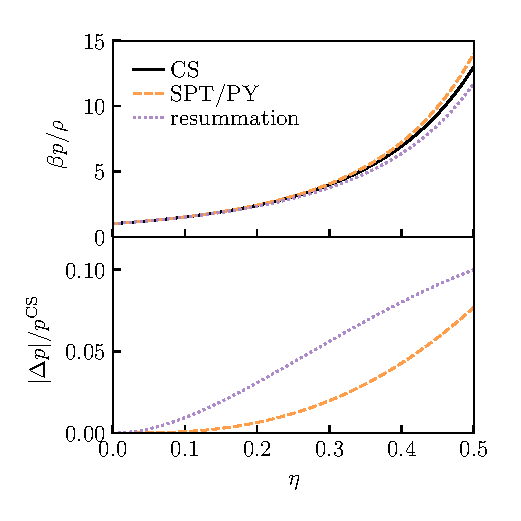
\includegraphics[width=0.9\linewidth,outer]{resummation-pressure}
  \caption[Accuracy of the equation of state obtained from partially resumming the virial series]{
    Equations of state for the single-component hard sphere liquid in $d=3$: Carnahan-Starling (CS), the scaled particle/Percus Yevick (SPT/PY) and the equation obtained from resumming terms in the virial series where there is a common point of intersection.
    Top panel: pressure equations of state.
    Bottom panel: errors in the SPT/PY and resummation pressures are comparable across the whole liquid regime, taking the CS equation as the quasi-exact result.}
  \label{fig:resummation-pressure}
\end{SCfigure}

Finally, for $d=3$ we insert \eqref{eq:little-lambda-d=3} into \eqref{eq:final-a-coefficient}:
\begin{subequations}
  \begin{align}
    \beta a_0 &= -\ln{(1 - \xi_3)},
    \\
    \beta a_1 &= \frac{2 \xi_2}{1-\xi_3},
    \\
    \beta a_2 &=
    2 \pi
    \left(
    \frac{\xi_1}{1-\xi_3}
    + \frac{\xi_2^2}{2(1-\xi_3)^2}
    \right),
    \\
    \beta p =
    \beta a_3 &=
    8 \pi
    \left(
    \frac{\xi_0}{1-\xi_3}
    + \frac{\xi_1 \xi_2}{(1-\xi_3)^2}
    + \frac{\xi_2^3}{3 (1-\xi_3)^3}
    \right).
    \label{eq:a3-d=3}
  \end{align}
\end{subequations}
For hard spheres of diameter $\sigma$ we obtain $V_1 = 2\sigma$ and $V_2 = \pi \sigma^2 / 2$ so $\xi_0 = \rho / (8\pi)$, $\xi_1 = \rho \sigma / (2\pi)$, $\xi_2 = \rho \pi \sigma^2 / 8$ and $\xi_3 = \eta$ for the single-component fluid.
This is similar but not identical to the Percus-Yevick equation of state%
\marginfootnote{Specifically via the compressibility route.
  See section \ref{sec:fmt} for a description of the single-component case.}
for additive mixtures, which in terms of this chapter's normalisations of the scaled particle variables reads \cite{Santos2016}
\begin{equation}\label{eq:py-pressure-mixtures}
  \beta p^\mathrm{PY} =
  8 \pi
  \left(
  \frac{\xi_0}{1-\xi_3}
  + \frac{\xi_1 \xi_2}{(1-\xi_3)^2}
  + \frac{16 \xi_2^3}{3 \pi^2 (1-\xi_3)^3}
  \right),
\end{equation}
which is exact up to the third virial coefficient $B_3$, and reduces to the SPT/PY equation \eqref{eq:py-pressure} in the case of single-component hard spheres.
By contrast, the resummation approach only provides a lower bound on $B_3$; the omitted configurations are known in the FMT literature as ``lost cases'' \cite{TarazonaPRE1997}.
A semi-empirical approach to obtain \eqref{eq:py-pressure-mixtures} could involve reweighting the final term in \eqref{eq:a3-d=3} to produce the exact third virial coefficient, giving an equation of state for arbitrary mixtures of convex particles.
This reweighting is implicit in scaled particle theory and the Rosenfeld FMT functional \eqref{eq:rosenfeld-functional} \cite{TarazonaPRE1997,MarechalPRE2014}.
In particular, scaled particle theory in $d=3$ is able to achieve accuracy at the $B_3$ level because of the additional constraint at the origin \eqref{eq:spt-point-d2} which is not available in $d=2$.
Such a reweighting approach is redundant because \eqref{eq:py-pressure-mixtures} and the Rosenfeld functional are already known, so this of fundamental rather than practical interest.

%Generically $V_d$ is the $d$-dimensional volume, so we will find $\xi_d = \eta$.

\section{Numerical results for the single-component hard spheres}

\begin{SCfigure}
  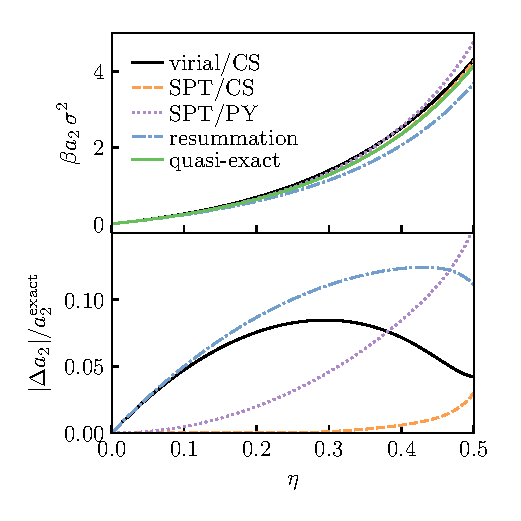
\includegraphics[width=0.9\linewidth,outer]{resummation-a2}
  \caption[Accuracy of surface tension obtained from partially resumming the virial series]{
    Comparison of surface tensions for different morphometric theories.
  using the highly accurate result \eqref{eq:quasi-exact-surface-tension} from Ref.\ \cite{DavidchackMP2015} valid until $\eta \sim 0.5$.}
  \label{fig:resummation-a2}
\end{SCfigure}

For single-component hard spheres the pressure obtained from the resummation in the previous section yields
\begin{equation}
  \frac{\beta p}{\rho} =
  \begin{cases}
    \frac{1}{1-\eta} & \; d=1 \\
    \frac{1}{(1-\eta)^2} & \; d=2 \\
    \frac{1 + \eta + (\frac{3\pi^2}{16} - 2) \eta^2}{(1-\eta)^3} & \; d=3.
  \end{cases}
\end{equation}
The resulting pressures for $d \le 2$ are identical to those obtained by scaled particle theory, where the first is actually exact \eqref{eq:hard-rods-eos}.
For $d=3$ the resulting equation of state has a similar structure to the scaled particle theory solution (or equivalently the Percus-Yevick equation of state by the compressibility route) (SPT/PY) but it is slightly less accurate: at the freezing point $\eta_f \simeq 0.494$ the PY equation overestimates the pressure by $\sim7\%$ while for the above equation this is underestimated by $\sim11\%$, taking the Carnahan-Starling (CS) equation of state \cite{CarnahanJCP1969} as an estimate of the exact value.
The three equations of state mentioned in $d=3$ are plotted together in Fig.\ \ref{fig:resummation-pressure} across the whole liquid regime in hard spheres.
While not exact, this shows that the morphometric contributions account for $\sim$90\% of the equation of state which may suggest why morphological thermodynamics has been found to be highly accurate for descriptions of the hard sphere liquid \cite{RothPRL2006,LairdPRE2012,BlokhuisPRE2013,UrrutiaPRE2014,Hansen-GoosJCP2014,RobinsonPRL2019}.
This is discussed in more detail in the context of FMT in \cite{MarechalPRE2014}, and is partially attributable to cancellations of terms omitted from the resummation.

We see similar accuracy in the predicted surface tension at an infinite planar wall determined by%
\marginfootnote{This is true up to a normalisation constant, as $a_2$ conjugates with the intrinsic volume $V_2$ rather than the area $A = 2V_2$.
  The usual planar surface tension is thus obtained as $\gamma_\infty = a_2/2$.}
$a_2$.
To measure accuracy we restate the quasi-exact result \eqref{eq:quasi-exact-surface-tension} of Ref.\ \cite{DavidchackMP2015} in terms of the normalisations used in this chapter as
\begin{equation}\label{eq:quasi-exact-surface-tension}
  %\begin{split}
  \beta a_2
  =
  \frac{2}{\pi \sigma^2} \left(
  \frac{\eta (2 + 3\eta - \frac{9}{5}\eta^2 - \frac{4}{5}\eta^3 - (5 \times 10^4) \eta^{20})}{(1 - \eta)^2}
  %% \right.
  %% \\
  %% &
  %% \left.
  %% \vphantom{\frac{1}{1}}
  - \ln{(1 - \eta)}
  \right).
  %\end{split}
\end{equation}
We also compare the values of $a_2$ predicted by other morphometric theories of \eqref{eq:cs-spt-coefficients} (SPT/CS, or equivalently the coefficients \eqref{eq:wbii-coefficients} of Ref.\ \cite{Hansen-GoosJPCM2006}) and the coefficients derived in chapter \ref{chapter:morphometric-framework} (virial/CS) given in \eqref{eq:virial-coefficients}.
The surface tensions are plotted in Fig.\ \ref{fig:resummation-a2}; the accuracy of the new result is comparable to SPT/PY in the liquid regime with the maximum error reaching $\sim12\%$.
Unsurprisingly, the other morphometric theories feature more accurate surface tensions; this is likely because they were constructed to satisfy thermodynamic relations which improves their accuracy.
%By contrast, the resummation route was not constructed for accuracy nor to satisfy thermodynamic relations.
Curiously, the error in the new theory scales almost identically to virial/CS theory at small $\eta$ even though it has the opposing sign; all of the previous morphometric theories overestimate the surface tension, whereas the resummation route underestimates it.

%% \subsection{Beyond convex geometries and the choice of dividing surface}
%% \label{sec:general-geometries}

%% \begin{figure*}
%%   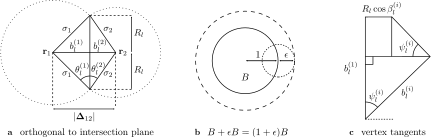
\includegraphics[width=0.65\linewidth,outer]{minkowski_addition}
%%   \caption{A dimer geometry considered in pair correlations in a fluid of $B$ particles showing (a) solute of two spheres $A$ generating an excluded volume $A \minkplus B$ and (b) the effective connected solute $A \minkplus B \minkminus B$.
%%   The exluded volume in each case is identical i.e.\ $A \minkplus B \minkminus B \minkplus B = A \minkplus B$.}
%%   \label{fig:minkowski_addition}
%% \end{figure*}

%% Until now we have focused on convex bodies, but we will now argue that the results apply for more general bodies.
%% In particular, for many-body correlations the ``solute'' consists of the disjoint union of particles see e.g.\ Fig.\ \ref{fig:system}.
%% We will determine necessary conditions for validity of the morphometric approach in in general solutes by examining the exact morphometric contributions described in previous sections.
%% A related problem is thermodynamic consistency for different choices of dividing surfaces in \eqref{eq:surface-tension}, which we will address in parallel.

%% Based on the exact results there are two ways the approach could fail:
%% \begin{enumerate}
%% \item For geometries where the integral geometric formula are invalid, e.g.\ the kinematic integrals, for non-convex geometries kinematic formula, and
%% \item Where the interaction with the solute cannot be reduced to the Euler characteristic, i.e.\ \eqref{eq:interactions-euler-equivalence}.
%% \end{enumerate}
%% As there are exact morphometric contributions to the free energy, a good approximation scheme should contain these; conversely, where these contributions are not captured provides necessary conditions for the scheme's validity.
%% We will address both potential failures in turn.

%% We used the kinematic integral \eqref{eq:binomial-kinematic-equation}, and its iterated form \eqref{eq:multinomial-kinematic-equation}, with convex bodies but it is valid for many more physically relevant geometries.
%% They can be extended \cite{Klain1997} to so-called \emph{polyconvex} bodies (also known as the convex ring), meaning any body formed by the countable union of convex objects.
%% This latter category covers most physically meaningful geometries, omitting pathological cases where size measures lose their meaning creating paradoxes \cite{BanachFM1924}.
%% The argument from Hadwiger's theorem similarly extends to polyconvex bodies.

%% Though the integral theorems hold for geometries of relevant physical interest, the equivalence between interaction and geometry \eqref{eq:interactions-euler-equivalence} may not.
%% We will consider two examples below in order to extend the geometric formalism to cases of physical interest.

%% First, consider the geometry formed by creating an infinitesimally small cavity inside a convex object.
%% Its Euler characteristic will deviate by $\pm 1$ (with sign dependent on dimension), however the interactions are unchanged because the cavity is not large enough to contain a finite-sized object.
%% In this case \eqref{eq:interactions-euler-equivalence} holds so long as the original convex geometry is used in place of the `true' body with the cavity.
%% %Going a step further, for finite-sized cavities able to contain a solvent particle, the cavity will be dynamically inaccessible to solvent particles (unless initially prepared inside) so the whole body can be treated as if it were solid, i.e.\ the interior of $\partial B$.

%% Next, we consider a geometry more typical of correlations in liquids: a dimer formed by two unit balls a distance $r$ apart i.e.\
%% \begin{equation*}
%%   A(r) = B^d \cup \mathcal{T}(r) B^d,
%% \end{equation*}
%% sketched in Fig.\ \ref{fig:minkowski_addition}.
%% This geometry is non-convex, and for $r > 1$ it is not even simply connected.
%% For interactions with a convex solvent particle $B$ we have possible Euler characteristics of intersection $\chi[A \cap B] \in \{0, 1, 2\}$ whereas $e^{-\beta u(A, B)} \in \{0, 1\}$, so it is not possible to establish an exact correspondence between the two.
%% We can proceed by determining an effective geometry where this relation does hold.
%% The exact result \eqref{eq:exact-mayer-exclusion} can be written
%% \begin{equation}
%%   \begin{split}
%%     e^{-\beta u(A, \mathcal{T} B)} - 1
%%     &= -\chi[(A \minkplus B) \cap \{\vec{r}\}] \\
%%     &= -\chi[(A \minkplus B \minkminus B) \cap B],
%%   \end{split}
%% \end{equation}
%% with the last line valid so long as $A \minkplus B \minkminus B = \{\vec{c} \, | \, (\vec{c} \minkplus B) \subseteq A \minkplus B\}$ is simply connected, otherwise the Euler characteristic of the intersecting geometry can be greater than one $\chi[(A \minkplus B \minkminus B) \cap B] > 1$.
%% The effective geometry $A \minkplus B \minkminus B$ recovers the correspondence between interaction and geometry \eqref{eq:interactions-euler-equivalence}.
%% Addition (dilation) and subtraction (erosion) operations are not inverse operations so $A \minkplus B \minkminus B \ne A$, however $A \minkplus B \minkminus B \minkplus B = A \minkplus B$ so $A \minkplus B \minkminus B$ acts as an effective generator of the exclusion region.
%% The effective geometry for the previous example, a nearly convex body with an infinitesimal cavity, recovers the convex object.

%% Related to the above discussion is the effect of the choice of dividing surface on the decomposition of surface and volume terms in \eqref{eq:surface-tension}.
%% The thermodynamics should not depend on the choice of boundary, i.e.\ we can define a functional working with the parallel surface
%% \begin{equation*}
%%   \Delta \Omega'[A \minkplus \epsilon B]
%%   =
%%   \sum_{k=0}^d a_k' V_k(A \minkplus \epsilon B)
%% \end{equation*}
%% but thermodynamic consistency requires
%% \begin{equation*}
%%   \Delta \Omega[A] =
%%   \Delta \Omega'[A \minkplus \epsilon B].
%% \end{equation*}
%% A controlled expansion of the solvation energy which allows for different choices of dividing surface must be invariant to the particular choice.
%% The transformation between the coefficients $\{a_k\}$ and $\{a'_k\}$, which we give explicitly in Appendix \ref{appendix:parallel-surfaces}, are straightforward which is a particular strength of using the morphometric \emph{ansatz}.
%% When this transformation fails leading to inconsistent thermodynamics, we know the theory has failed.
%% We find a necessary condition for the theory's validity is thus that $\chi[A \minkplus B^d \minkminus B^d] = \chi[A \minkplus B^d]$.

%% The boundary of the effective volume $\partial(A \minkplus B \minkminus B)$ is commonly called the \emph{molecular surface} \cite{?}, while the boundary of the excluded volume $\partial(A \minkminus B)$ is referred to as the \emph{solvent accessible surface}.
%% There is also an infinite family of equivalent parallel surfaces in between i.e.\ $\partial(A \minkplus B \minkminus \epsilon B)$ for $\epsilon \in [0, 1]$ but the two extremes are the most natural choices.
%% When the boundary of the effective geometry (molecular surface) self-intersects, we expect the theory to break down.
%% In the previous example this occurs at $r = 2\sqrt{3}$ for spherical solvent particles $B = B^d$ \cite{OettelEL2009}.
%% At this point, descriptions with different choices of boundary become inconsistent.
%% Consider the Euler characteristic of the effective body (molecular surface)
%% \begin{equation}
%%   \chi[A \minkplus B^d \minkminus B^d]
%%   =
%%   \begin{cases}
%%     1 & r < 2\sqrt{3} \\
%%     2 & r > 2\sqrt{3}
%%   \end{cases}
%% \end{equation}
%% whilst for the parallel volume (solvent accessible surface)
%% \begin{equation}
%%   \chi[A \minkplus B^d]
%%   =
%%   \begin{cases}
%%     1 & r < 2 \\
%%     2 & r > 2
%%   \end{cases}
%% \end{equation}

\section{Conclusions}

We have derived an exact morphometric contribution for a general class of hard particle liquids by resumming terms in the virial series.
Previous studies have primarily used FMT to develop morphometric theories, so we have successfully developed an independent justification for the morphometric approach as the leading term in a controlled expansion.
The exact result applies for mixtures of hard convex particles in an isotropic phase.

%This result is not that surprising as the morphometric approach can be obtained as a limit case of FMT \cite{Hansen-GoosJPCM2006}, which itself can be formulated as the resummation of the same terms in the virial expansion \cite{LeithallPRE2011,KordenPRE2012,MarechalPRE2014}.

In hard spheres, this exact contribution features similar accuracy as scaled particle theory, and exactly coincides with it for $d \le 2$.
Numerical comparison in $d=3$ shows that the pressure and surface tension are comparable in accuracy to the classic SPT/PY route, so it captures the dominant contributions to the bulk free energy across a large density range; this latter fact seems to suggest why the approach has been successful.
Though as noted in Ref.\ \cite{MarechalPRE2014}, this is partially due to a cancellation in the omitted terms of the virial expansion.%, so it may still be desirable to improve the morphometric approach by inclusion of additional terms.
%We have derived the morphometric solvation free energy for mixtures of hard convex particles from first-principles using the virial series.
%% The morphometric theory we have derived from the virial series is less accurate than theories obtained from other routes, so these results are of fundamental rather than practical interest.
%% Specifically, in $d=3$ the pressure and surface tension are comparable in accuracy to the classic SPT/PY route, and in $d=2$ the approach is identical to scaled particle theory.
The usefulness of the new route extends beyond mere accuracy; the free energy we have identified emerges \emph{rigorously} as a contribution from the virial series.

The fact that the exact contribution is reasonably accurate suggests that the corrections are small, providing further justification of the morphometric approach.
Moveover, the exact contribution provides a suitable starting point for including additional terms to improve accuracy.
We could write the insertion cost for a solute $K$ as the \emph{exact} decomposition
\begin{equation}\label{eq:exact-morph-decomposition}
  \Delta \Omega[K]
  =
  \sum_{k=0}^d a_k V_k[K]
  + \Delta \Omega_\mathrm{extra}[K]
\end{equation}
with coefficients $a_k$ as previously calculated, and $\Delta \Omega_\mathrm{extra}$ contains the subleading corrections.
Notably, the exponentially damped oscillations occuring in pair correlations at asymptotically large separations must be contained within $\Delta \Omega_\mathrm{extra}$.
The insertion cost is known to contain singularities%
\marginfootnote{See Appendix \ref{appendix:spt-singularities} where we recount an old argument from Ref.\ \cite{ReissJCP1959} that $\Delta \Omega$ contains singularities.}
so it is unlikely that $\Delta \Omega_\mathrm{extra}$ possesses a simple analytic form.
It is possible that additional exact morphometric contributions exist, and they would be contained in $\Delta \Omega_\mathrm{extra}$ also.

Furthermore, the formal derivation we have followed naturally leads to explicit expressions for $\Delta \Omega_\mathrm{extra}$.
The next leading contribution from the virial series would be:
\begin{equation}
  \begin{split}
    \Delta \Omega_\mathrm{extra}[K]
    =&
    \frac{\rho^2}{2}
    \sum_{s_1=1}^m \sum_{s_2=1}^m
    x_{s_1} x_{s_2}
    \left(
    \Delta_{s_1,s_2}
    %% \int_{G_d^2} \chi[K \cap g_1 K_{s_1}]
    %% \right.
    %% \\
    %% &
    %% \left.
    %% \chi[K \cap g_2 K_{s_2}] \chi[g_1 K_{s_1} \cap g_2 K_{s_2}] dg_1 dg_2
    - \Lambda_{s_1,s_2} \right)
    + \mathcal{O}(\rho^3),
  \end{split}
\end{equation}
where $\Delta_{s_1,s_2}$ is the three-body \emph{ring integral} given explicitly in the first line of \eqref{eq:ring-integral-3}.
%% \begin{equation}\label{eq:ring-integral-3}
%%   \Delta_{s_1,s_2}
%%   =
%%   \int_{G_d^2}
%%   \chi[K \cap g_1 K_{s_1}] \, \chi[K \cap g_2 K_{s_2}] \, \chi[g_1 K_{s_1} \cap g_2 K_{s_2}]
%%   \, dg_1 dg_2.
%% \end{equation}
Ring integrals can be calculated straightforwardly in hard spheres \cite{MontrollJCP1941}, or using the Radon transform for convex geometries of arbitrary shapes \cite{WertheimMP1994,WertheimMP1996,WertheimMP1996a}.
Corrections to the morphometric approximation could be systematically included by further resummations over classes of diagrams, with ring integrals as the leading order terms.
The integral corrections are discussed in Ref.\ \cite{MarechalPRE2014} in the context of free energy functionals for inhomogeneous liquids; our system is effectively homogeneous so we expect it to be easier to construct a theory with these higher-order terms.
Notably, the ring integrals are argued to be the sole contributions in the mean-field infinite-dimensional limit, i.e.\ for a single-component system \cite{ParisiRMP2010}
\begin{equation*}
  \lim_{d \to \infty}
  \frac{\beta F_{ex}}{V}
  =
  \rho^2 \mayerdiagram[|][t.]{2} +
  \rho^3 \mayerdiagram[|||][t..]{3} +
  \rho^4 \, \mayerdiagram[|.||.|][t...]{4} +
  \rho^5 \; \mayerdiagram[|..||..|.|][t....]{5} +
  \mathcal{O}(\rho^6),
\end{equation*}
ignoring combinatorial prefactors for clarity.
The equivalent diagrams in the morphometric/FMT approaches are given in \eqref{eq:fmt-diagrams}.
Resumming the ring diagrams would lead to a contribution in $\Delta \Omega$ involving a double volume integral over the solute geometry, and their inclusion could possibly provide more of a connection between the morphometric approach and the results of mean-field hard sphere calculations (section \ref{sec:mean-field-glass}).

The form of the exact contribution is instructive in how it applies to mixtures.
It is argued in Ref.\ \cite{KodamaJCP2011} that for an $m$-component mixture the appropriate morphometric form reads
\begin{equation}\label{eq:morphometric-approach-mixtures}
  \Delta \Omega[K]
  =
  \sum_{i=1}^m
  a_3^{(i)} V_i[K]
  + a_2^{(i)} A_i[K]
  + a_1^{(i)} C_i[K]
  + a_0^{(i)} X_i[K]
\end{equation}
where the coefficients $a_k^{(i)}$ now depend on the specific interactions with each species and their composition, and $\{V_i, A_i, C_i, X_i\}$ are geometric measures on some composite body of the solute with solvent particles of species $i$, e.g.\ their specific exluded volume.
By contrast, our exact morphometric contribution does not involve different intrinsic volumes for the different cross-species interactions, suggesting \eqref{eq:morphometric-approach-d} is a general enough \emph{ansatz} and the extension for mixtures \eqref{eq:morphometric-approach-mixtures} proposed in Ref.\ \cite{KodamaJCP2011} may be unnecessary.
Moreover, as functions of the scaled particle variables $\{\xi_i\}$ the coefficients we derive remain well-defined in the polydisperse limit $m \to \infty$, discussion of which can be found in section \ref{sec:truncatable-free-energy} and in more detail in Refs.\ \cite{GualtieriJCP1982,WarrenPRL1998,SollichPRL1998,SollichAiCP2001}.
With the number of coefficients growing with $m$ in \eqref{eq:morphometric-approach-mixtures}, it is unclear how well-posed this \emph{ansatz} is in that limit.

\ifdefined\includebibliography
  \newgeometry{margin=1in}
  \printbibliography
\fi

\end{document}
